\subsection{\href{https://www.disenioconingenio.com.ar}{disenioconingenio}}
   \hypertarget{subsec:dci}
   When I was in charge of Disenioconingenio, I developed several products for sale in the market and customized according to the characteristics required by the customers, the following stand out:\\
   \cvlistitem{RFID 125Khz Multiprotocol}
A 125khz RFID card reader was designed with a discrete frontend and fully decoded by the microcontroller. This allows reading data from different manufacturers and different protocols, and combining with multiple data outputs, such as RS232, RS485, Wiegand and ABA.\\
   There are shown some pictures in the figure \ref{fig:rfid}.
   \begin{figure}
      \begin{center}
         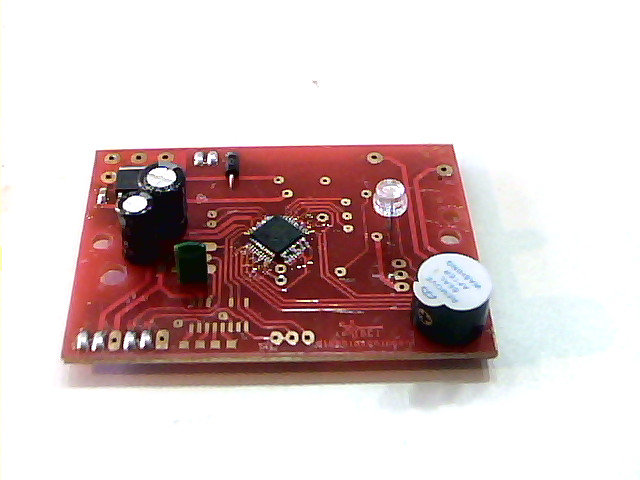
\includegraphics[width=0.24\textwidth]{rfid5.jpg}
         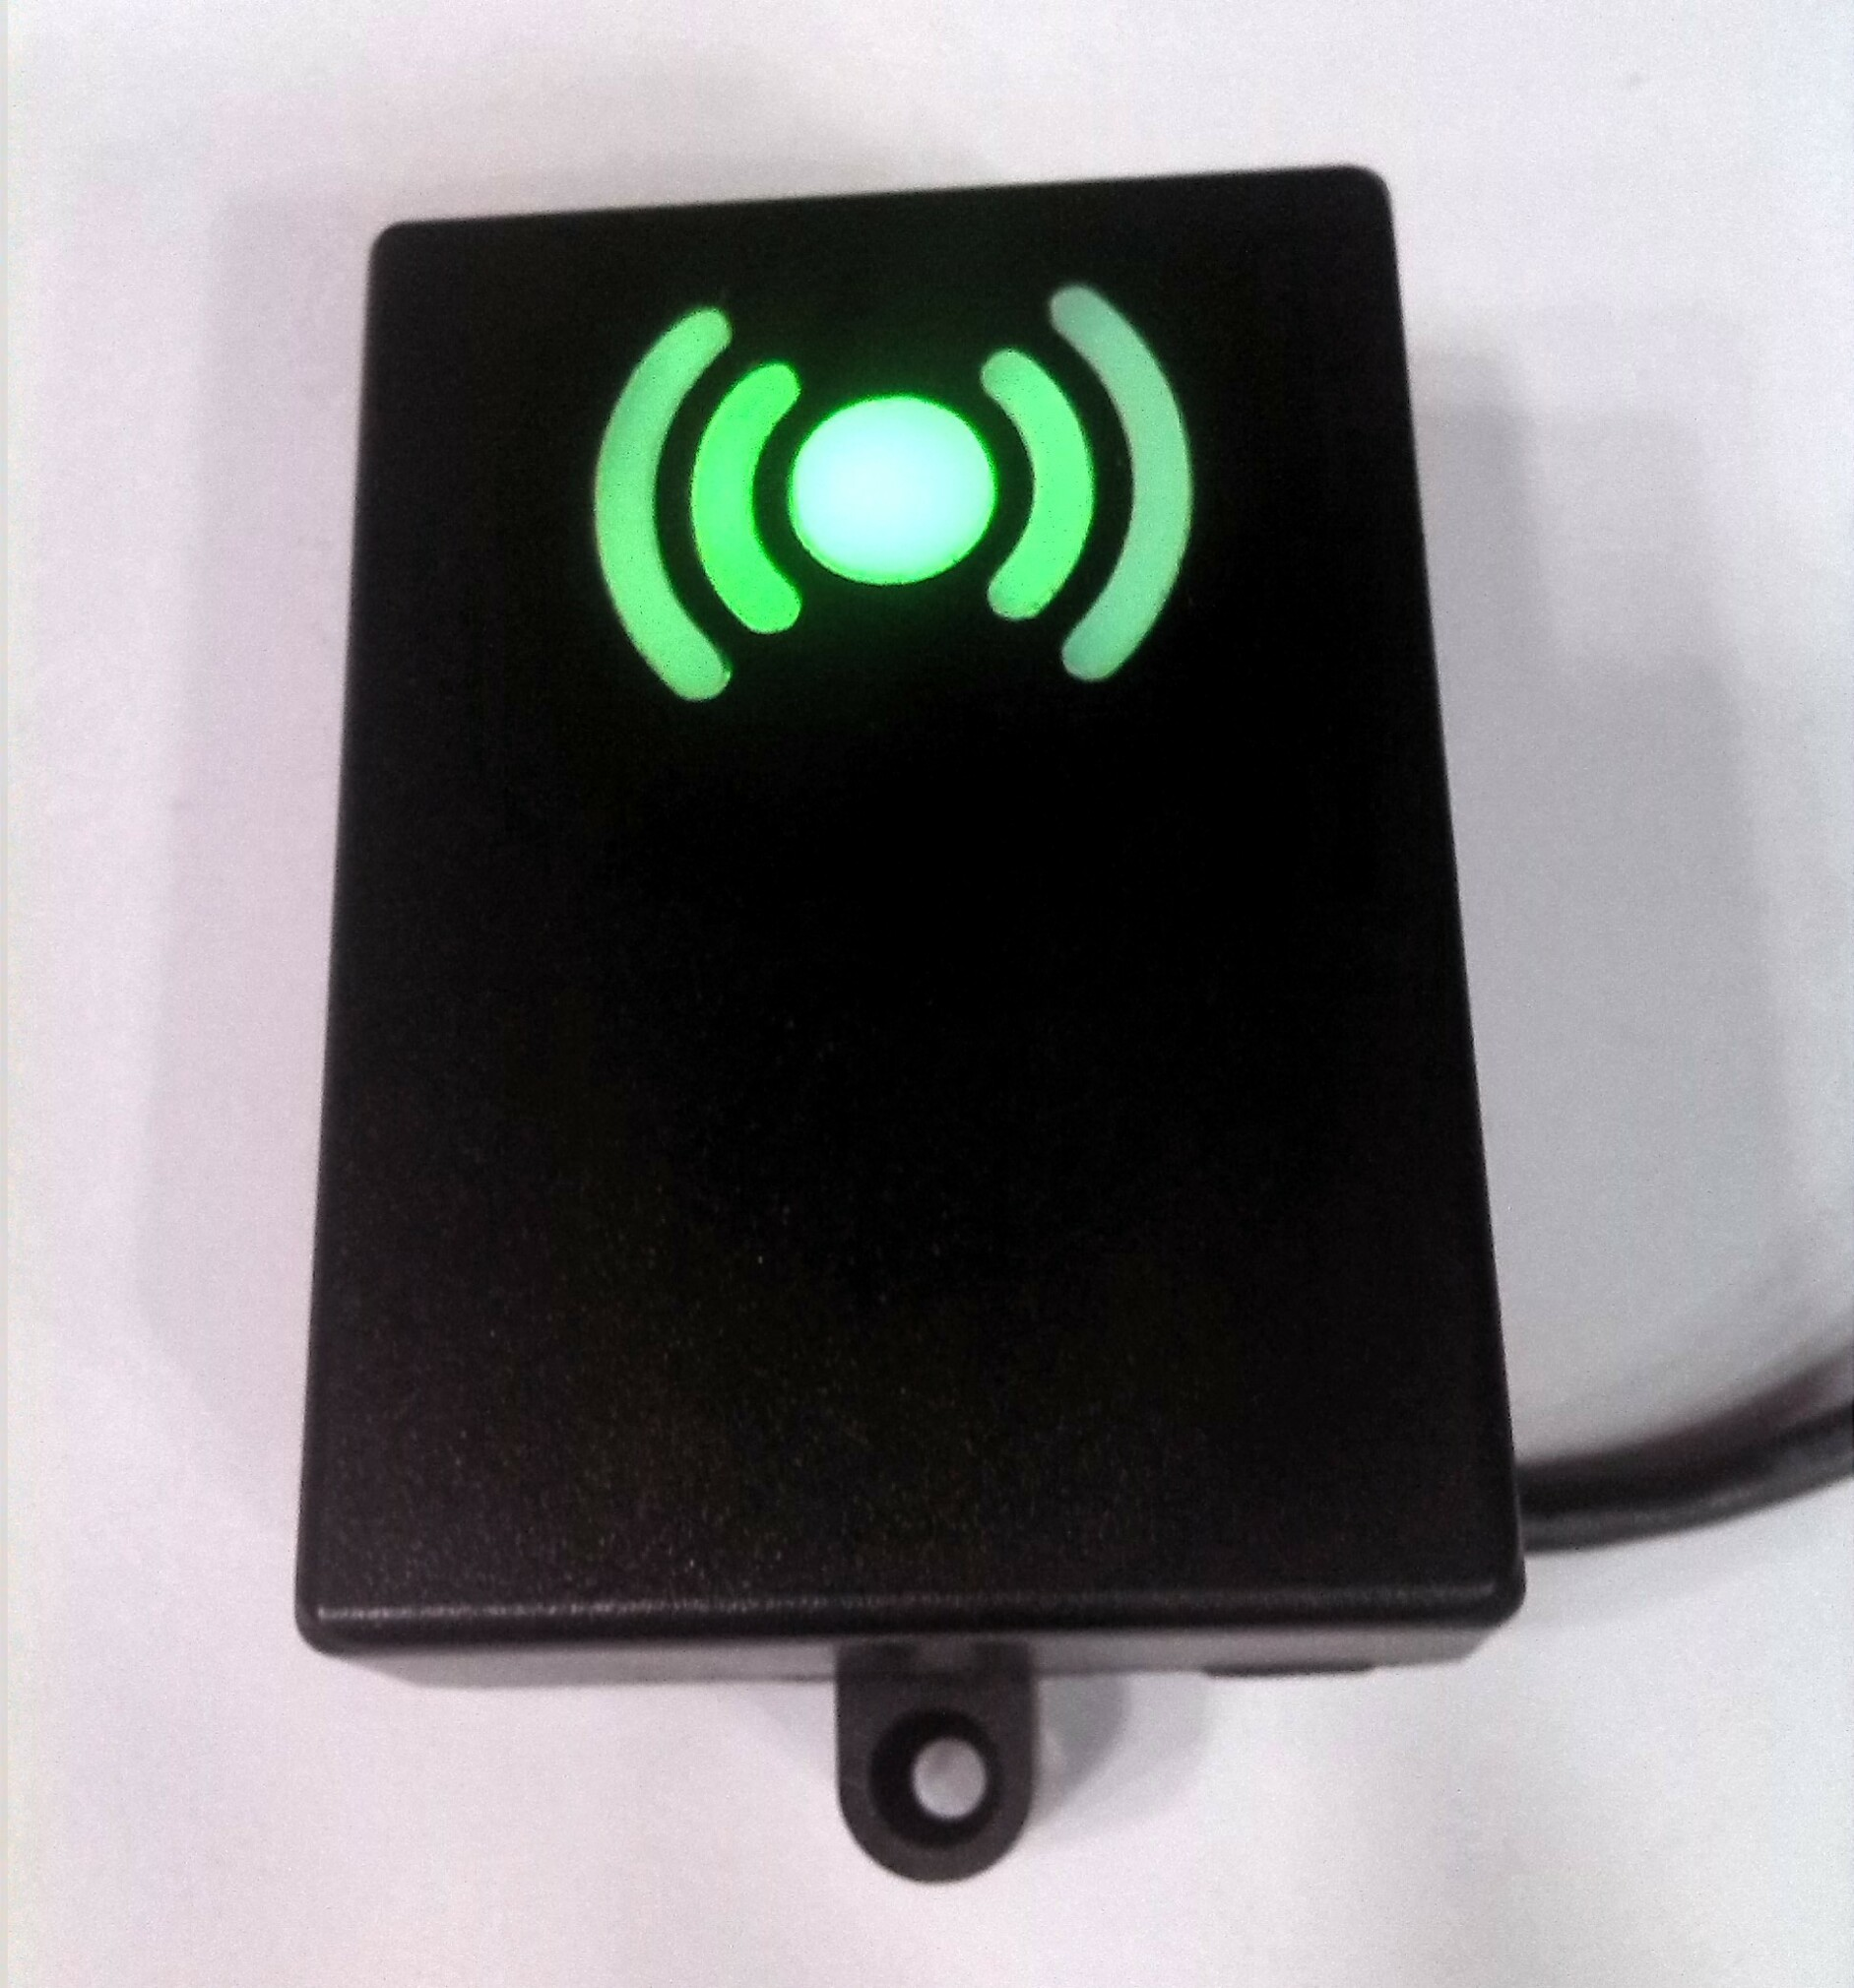
\includegraphics[width=0.24\textwidth]{rfid2.jpg}
         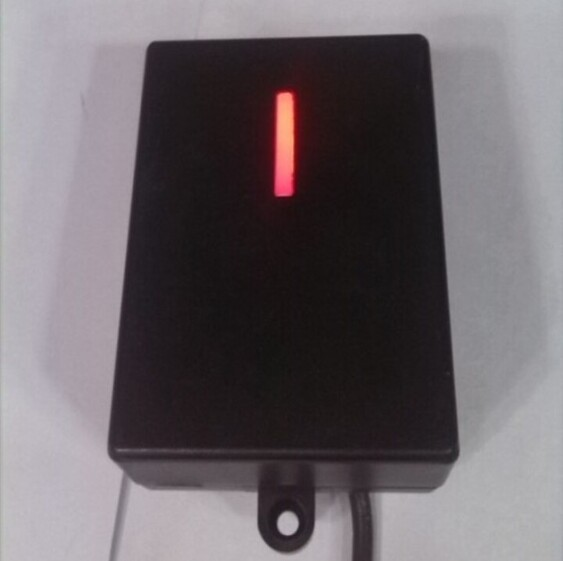
\includegraphics[width=0.24\textwidth]{rfid3.jpg}
         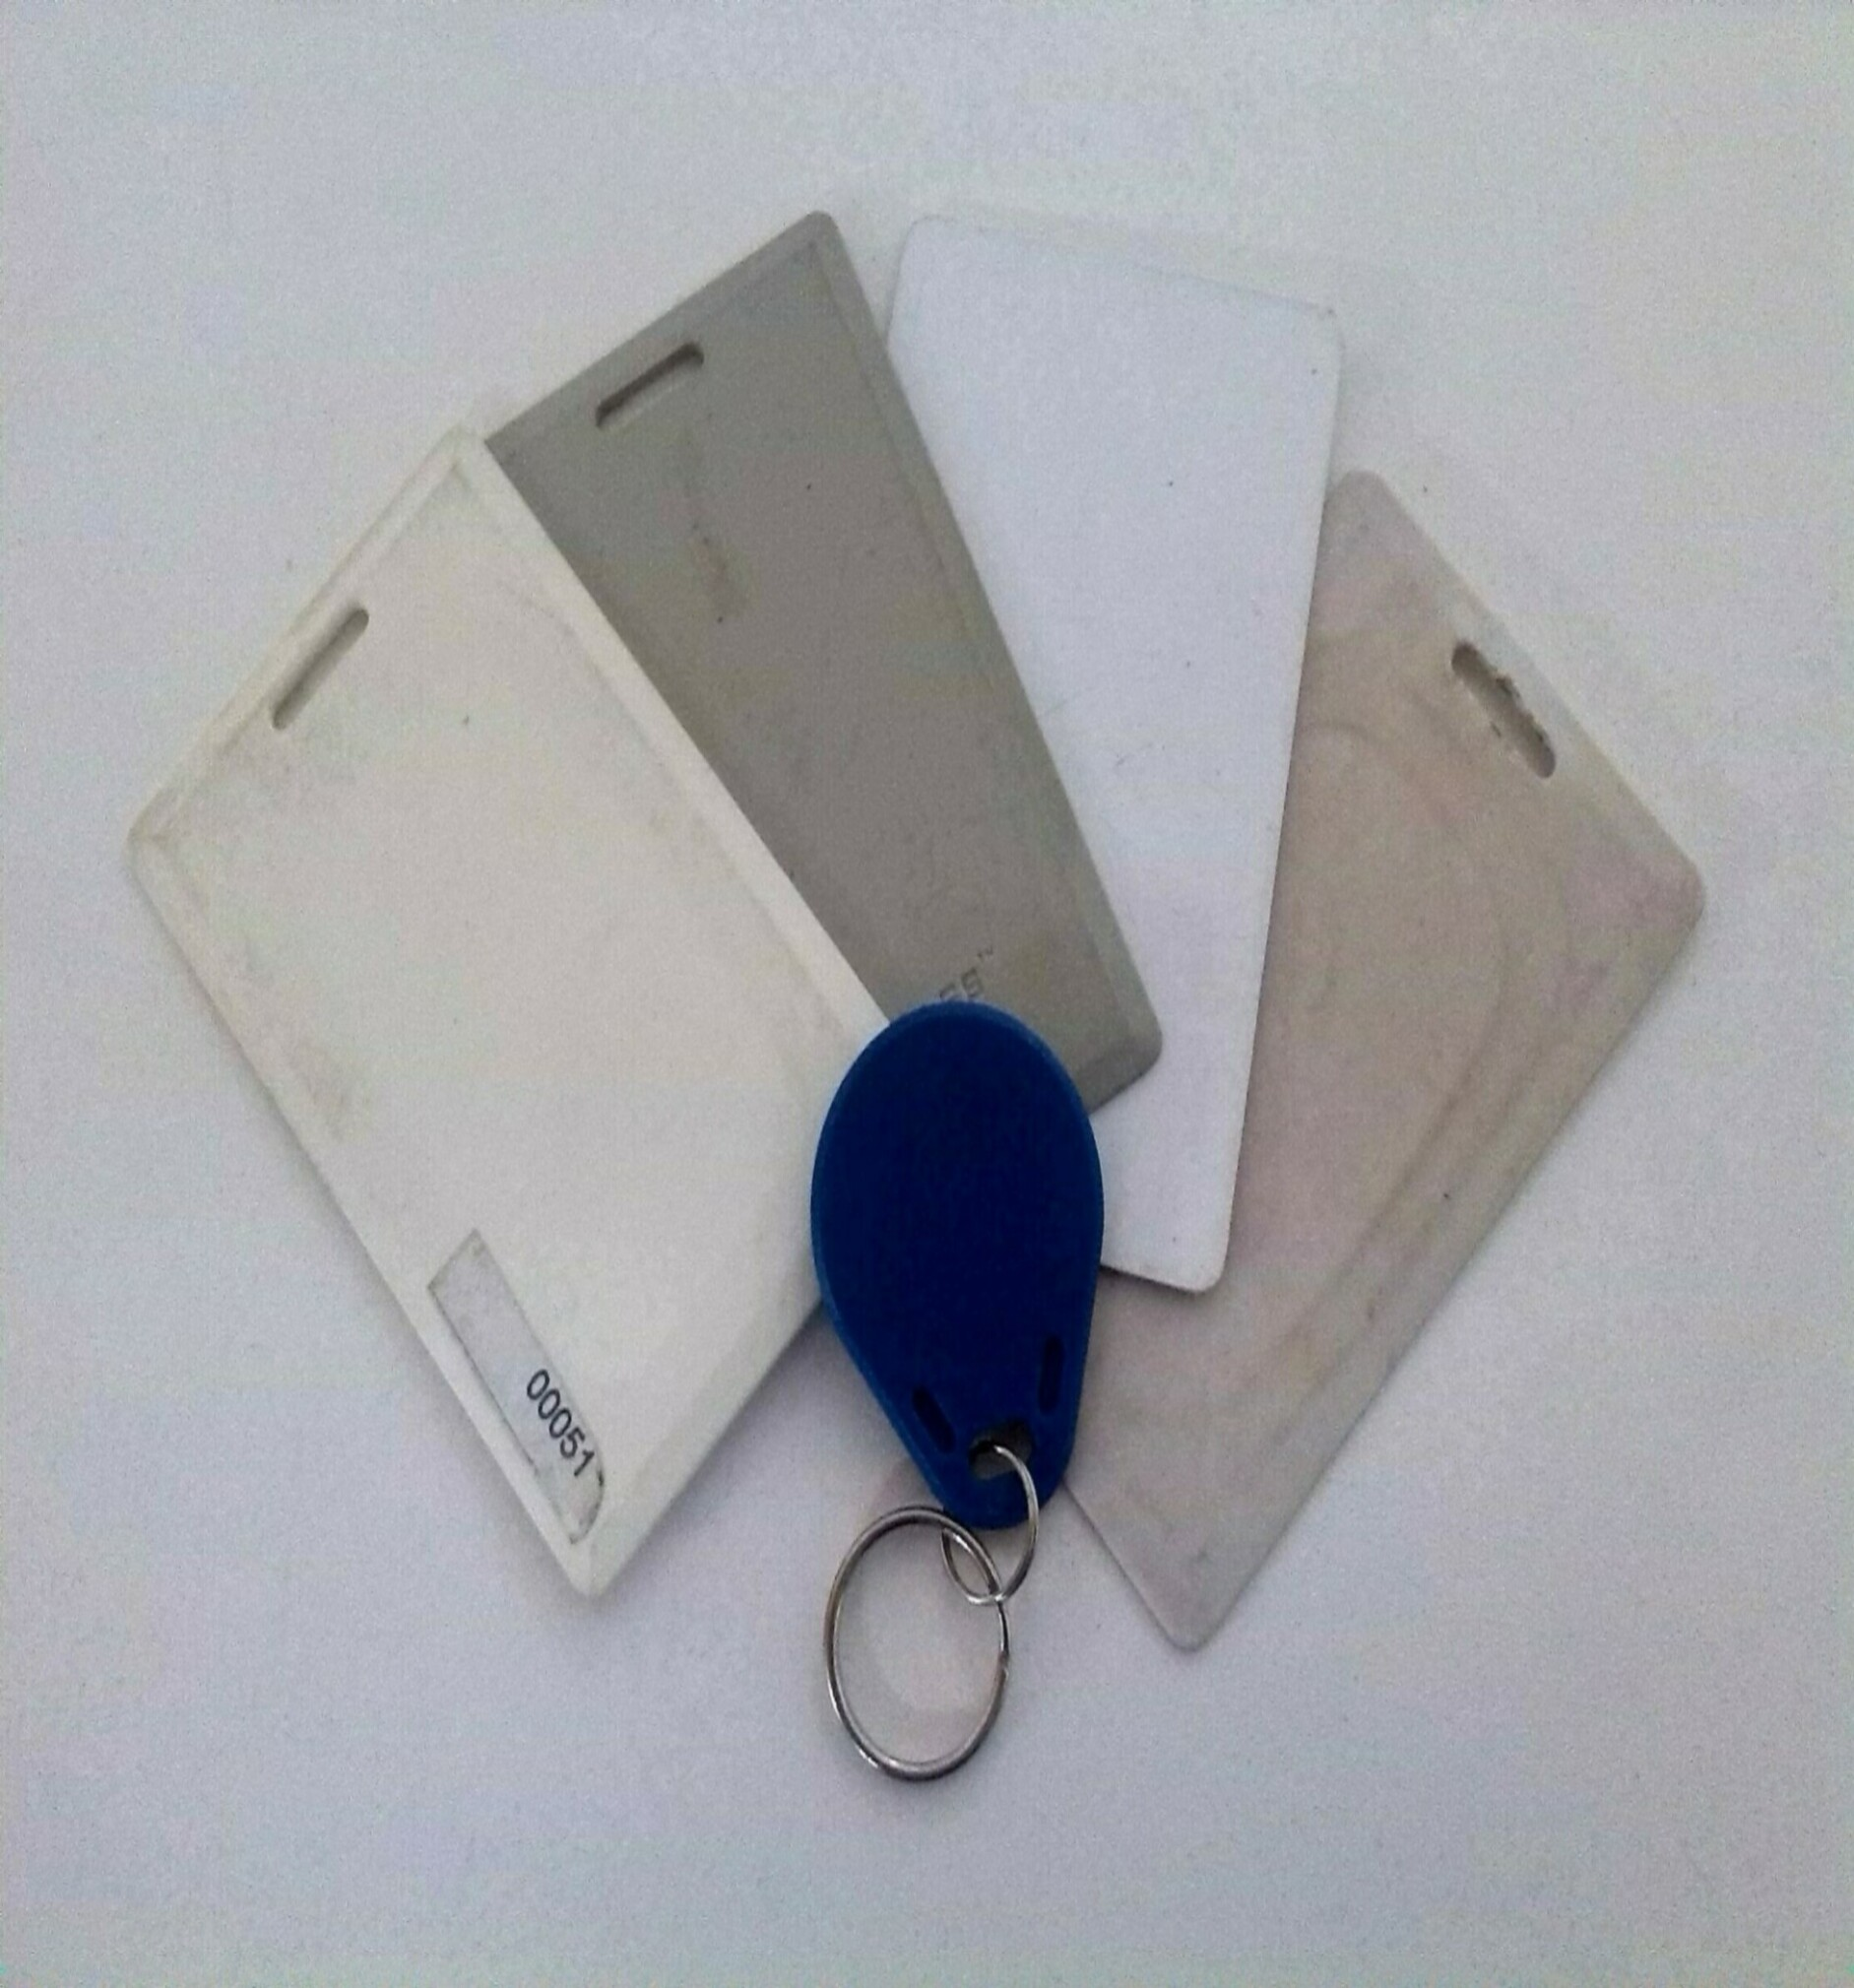
\includegraphics[width=0.24\textwidth]{rfid4.jpg}
      \end{center}
      \caption{125khz RFID multiplrotol card reader, compatible with most card manufacturers.}
      \label{fig:rfid}
   \end{figure}

   \cvlistitem{Hango - Wheel chair motorizer}
In conjunction with institutions dedicated to assisting people with mobility difficulties such as CIAPAT, AEDIN and FAME, we develop Hango.\\
   It consists of a motorizer that attaches to manually driven wheelchairs granting comfort and independence.\\
Models for children and adults up to 100kg were developed with different styles of commands, some based on the typical joystick, and other new ones using touch screen technology.\\
   The equipment adapts to the vast majority of market chairs with minimal mechanical intervention and allows the coupling and uncoupling without tools, suitable for transfers by car and plane.\\
Threr are some pictures in the figure \ref{fig:hango1} and \ref{fig:hango2} and also some videos at \href \linkhangovideos {Videos Hango}.
   \begin{figure}
      \begin{center}
         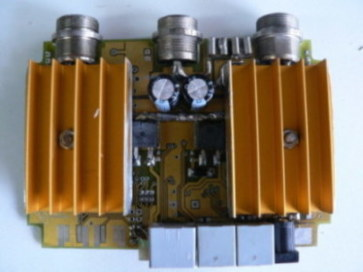
\includegraphics[width=0.24\textwidth]{hango1.jpg}
         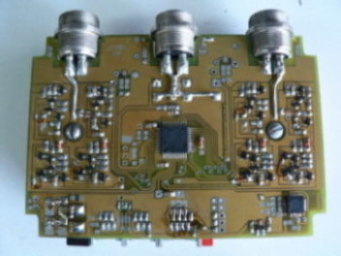
\includegraphics[width=0.24\textwidth]{hango2.jpg}
         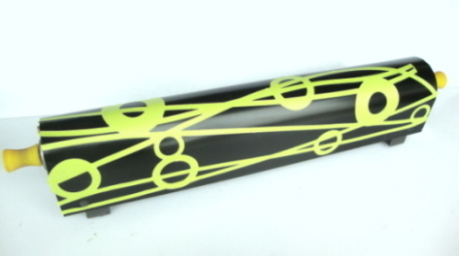
\includegraphics[width=0.24\textwidth]{hango3.jpg}
         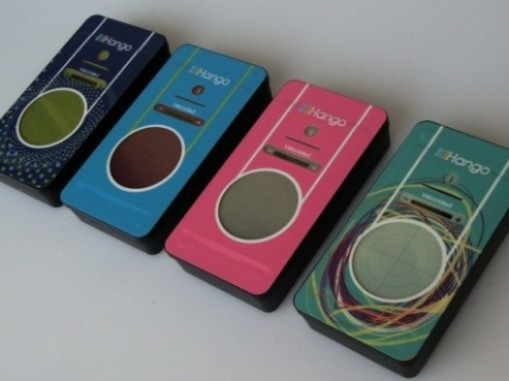
\includegraphics[width=0.24\textwidth]{hango4.jpg}
      \end{center}
      \caption{Hango Power boards, controller and joysticks.}
      \label{fig:hango1}
   \end{figure}
   \begin{figure}
      \begin{center}
         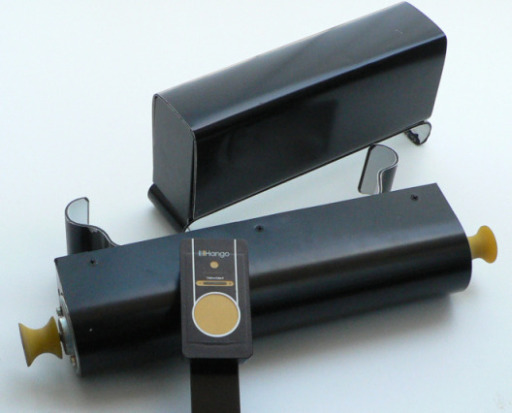
\includegraphics[width=0.24\textwidth]{hango5.jpg}
         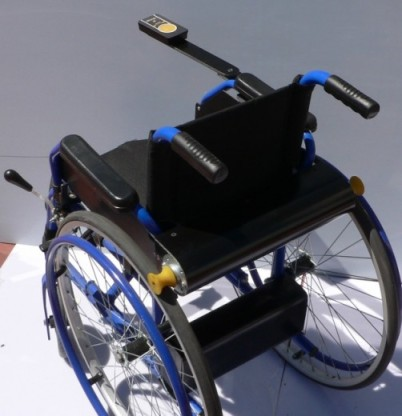
\includegraphics[width=0.24\textwidth]{hango6.jpg}
         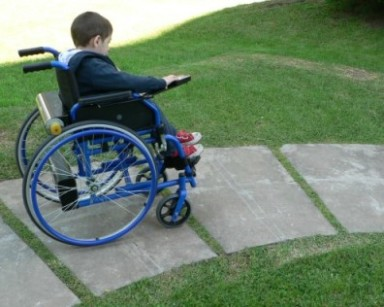
\includegraphics[width=0.24\textwidth]{hango7.jpg}
         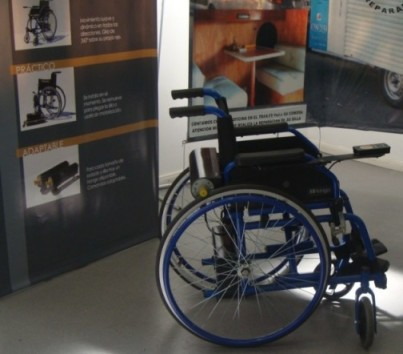
\includegraphics[width=0.24\textwidth]{hango8.jpg}
      \end{center}
      \caption{Hango parts, and Hango at the CIAPAT expo.}
      \label{fig:hango2}
   \end{figure}
